% Это основная команда, с которой начинается любой \LaTeX-файл. Она отвечает за тип документа, с которым связаны основные правил оформления текста.
\documentclass{article}

% Здесь идет преамбула документа, тут пишутся команды, которые настраивают LaTeX окружение, подключаете внешние пакеты, определяете свои команды и окружения. В данном случае я это делаю в отдельных файлах, а тут подключаю эти файлы.

% Здесь я подключаю разные стилевые пакеты. Например возможности набирать особые символы или возможность компилировать русский текст. Подробное описание внутри.
\usepackage{packages}

% Здесь я определяю разные окружения, например, теоремы, определения, замечания и так далее. У этих окружений разные стили оформления, кроме того, эти окружения могут быть нумерованными или нет. Все подробно объяснено внутри.
\usepackage{environments}

% Здесь я определяю разные команды, которых нет в LaTeX, но мне нужны, например, команда \tr для обозначения следа матрицы. Или я переопределяю LaTeX команды, которые работают не так, как мне хотелось бы. Типичный пример мнимая и вещественная часть комплексного числа \Im, \Re. В оригинале они выглядят не так, как мы привыкли. Кроме того, \Im еще используется и для обозначения образа линейного отображения. Подробнее описано внутри.
\usepackage{commands}


% Здесь я настроил пакет listings для отображения кода C++. Можно пользоваться непосредственно самим пакетом listings, но если вы про него ничего не знаете, то моя надстройка будет удобной стартовой точкой.
\usepackage{code}


\author{Дима Трушин}
\title{Материалы к программным проектам}
\date{}

% С этого момента начинается текст документа
\begin{document}

\maketitle

% Здесь будет автоматически генерироваться содержание документа
\tableofcontents

\begin{abstract}
Сразу дисклеймер, я не являюсь профессиональным программистом, я -- математик, который что-то понимает в программировании и Computer Science. Я постарался собрать в этом тексте какие-то наиболее полезные вещи, которые мне встретились за время работы над программными проектами на ПМИ ФКН. Я так же постарался добавлять ссылки на более подробное обсуждение затронутых вопросов или полезные материалы.
\end{abstract}


\section{Полезные ссылки}

\begin{itemize}
\item Прежде всего надо не забывать про \href{https://en.cppreference.com/w/}{cppreference} и \href{https://www.cplusplus.com/}{cplusplus}.

\item Кроме этого есть \href{https://isocpp.org/faq}{FAQ} по плюсам с кучей полезной информации по разным вопросам.

\item \href{https://wiki.sei.cmu.edu/confluence/pages/viewpage.action?pageId=88046682}{Guide} от SEI CERT по написанию надежного и безопасного кода на C и C++. 

\item Мой персональный \href{https://www.youtube.com/playlist?list=PL9ZoDZ0U4QLDyBOaf4biYoFd-TIly-Nhe}{плейлист} с полезными видео в основном по плюсам.
\end{itemize}

\section{Код на плюсах}

\subsection{Модель компиляции C++}

В C++ используется так называемая двух ступенчатая модель компиляции (реальных этапов компиляции там дофига, про все стадии можно почитать \href{https://en.cppreference.com/w/cpp/language/translation_phases}{тут}):
\begin{enumerate}
\item Этап компиляции в бинарные файлы.
\item Этап линковки бинарных файлов в исполняемый файл программы.
\end{enumerate}
Это две независимые стадии, которые выполняются разными программами. Давайте я на модельном примере поясню, что это все значит, и как понимать компиляцию плюсов. Предположим у вас есть следующие файлы:
\begin{cppcode}
// function.h

void function();

// function.cpp

#include "function.h"

void function() {
}

// main.cpp

#include "function.h"

int main() {
  function();
  return 0;
}
\end{cppcode}
Теперь надо провести компиляцию и линковку кода командами\footnote{Я использую условные команды и не использую синтаксис конкретных комиляторов и линкеров.}
\begin{enumerate}
\item compile \verb"function.cpp" to \verb"function.bin"
\item compile \verb"main.cpp" to \verb"main.bin"
\end{enumerate}
Во время первой команды компиляции \verb"function.cpp" создается так называемая единица трансляции. По простому, выполняются команды препроцессора и вставляются все \verb"#include" копипастой. То есть получается файл
\begin{cppcode}
// TU for function.cpp

void function();

void function() {
}
\end{cppcode}
После чего создается бинарный файл, скажем, \verb"function.bin", в который складывается информация о функциях и переменных из единицы трансляции.\footnote{Я не использую конкретный синтаксис ассемблера, я пишу условный машинный код.}
\begin{cppcode}
// function.bin

function:
  return;
\end{cppcode}

Теперь выполняется компиляция \verb"main.cpp". В начале составляется единица трансляции.
\begin{cppcode}
// TU for main.cpp

void function();

int main() {
  function();
  return 0;
}
\end{cppcode}
Теперь эта единица трансляции компилируется в машинный код.
\begin{cppcode}
// main.bin

main:
  call function();
  return 0;
\end{cppcode}

Обратите внимание, что компилятору не нужно знать определение \verb"function". Ему достаточно знать, что имя \verb"function" является именем функции и что \verb"function()" -- это вызов функции. Об этом компилятору сообщает строчка $3$ в единице трансляции для \verb"main.cpp". Без этой строчки \verb"function" было бы неизвестным именем и вызывало бы ошибку компиляции. А так это функция, которую компилятор не знает, но знает все, чтобы в \verb"main.bin" поместить правила ее вызова.

Теперь у нас есть два бинарных файла
\begin{cppcode}
// function.bin

function:
  return;
  
// main.bin

main:
  call function();
  return 0;
\end{cppcode}
И нам нужно вызвать линковку командой
\begin{itemize}
\item Link \verb"function.bin" and \verb"main.bin" to \verb"main.exe"
\end{itemize}
Точкой входа в программу является функция \verb"main()". Потому компилятор найдет ее и начнет из всех бинарников подставлять все необходимые функции. Мы видим, что внутри \verb"main" есть вызов функции \verb"function()". Для этого линкер должен где-то среди всех бинарников найти одну единственную функцию \verb"funcion()" и добавить ее код в \verb"main.exe". В итоге получится следующее
\begin{cppcode}
// main.exe

main:
  call function();
  return 0;
  
function:
  return;
\end{cppcode}
Если линкер не находит имени \verb"function()" ни в одном бинарнике -- это ошибка линковки. Если линкер находит две функции \verb"function" в разных бинарниках, то это тоже ошибка линковки, кроме специальных случаев.\footnote{К специальным случаям относятся функции помеченные словом \verb"inline" и инстанциации шаблонов, о которых я поговорю позже.} В специальных случаях мы должны гарантировать линкеру, что все определения для \verb"function" являются одинаковыми, потому что он может выбрать любое из них взамен другого. Соответственно, если это не так, то это undefined behavior.

Для чего сделано такое безобразие? Расчет в такой модели сделан на следующую организацию кода. Единицей кода является файл. И мы специально делим проект на несколько файлов, чтобы в случае внесения изменений нам не надо было перекомпилировать все файлы целиком, а лишь перекомпилировать один-два файла, и потом перелинковать нужные бинарники. Эта идея помогала значительно сократить время компиляции для больших проектов. Такая модель использовалась C, и потому плюсы переняли ее, добавив свои дополнительные стадии. Однако, файл, как единица компиляции, это очень плохая идея, особенно учитывая, что в плюсах появились шаблоны. Они как раз и ломают всю идиллию такого подхода.

\paragraph{Что нужно знать компилятору}

Обратите внимание, что в плюсах есть два понятия declaration и definition. Declaration -- это объявление объекта, которое говорит компилятору, что это за объект (переменная, функция, имя класса, имя шаблона и т.д.). Declaration может быть не достаточно для того, чтобы полностью скомпилировать код с этим объектом. Definition -- это declaration, которое полностью определяет объект. Например
\begin{cppcode}
void f(); // declaration

void f() {} // definition

static int x; // declaration

static int x = 1; // definition

class A; // declaration

class A {}; // definition

int y; // definition
\end{cppcode}
В строчке 1 мы видим declaration для функции. Его не достаточно, чтобы поместить в бинарник код для функции. Однако, его достаточно, чтобы поместить в бинарник точку вызова функции. В строчке 3 идет defintion для функции, его достаточно, чтобы поместить в бинарник код функции. В строчке 5 идет declaration для статической переменной. Чудесатость таких переменных заключается в том, что эта строчка не помещает переменную в память и не дает ей адрес, но говорит, что имя \verb"x" означает имя переменной типа \verb"int". А вот строчка 7 уже полностью определяет \verb"x" и после нее у \verb"x" появляется адрес. Строчка 9 -- declaration для класса. Ее не достаточно, чтобы создать переменную класса \verb"A", однако ее достаточно, чтобы создать указатель на этот класс, потому что все указатели имеют одинаковый размер. Строчка 11 -- definition для класса \verb"A" и ее уже достаточно, чтобы создать объект этого класса, мы точно знаем какой размер должен занять этот объект. Обратите внимание, что объявление не статической переменной на строке 13 является definition, потому что позволяет полностью определить объект с именем \verb"y" и работать с ним, хранить его в памяти и брать его адрес.

Как мы видели выше на модельном примере, модель компиляции плюсов построена вокруг идеи, что во время компиляции функций, если мы знаем ее определение (definition), то мы его добавляем в бинарник, а если не знаем, то добавляем в бинарник точку вызова этой функции. Главное -- надо знать, что имя действительно было именем функции. Для этого мы делаем \verb"#include" header-а содержащего declaration для имени функции. А тело функции будет компилировать в отдельной единице трансляции. И уже задача линкера найти нужное тело функции.

\subsection{Шаблоны и модель компиляции плюсов}

А теперь добро пожаловать в мир интересных интересностей -- шаблоны. 

\paragraph{Что такое шаблоны}
Прежде всего отмечу, что бывают шаблоны функций, классов и переменных.
\begin{cppcode}
template<class T>
void f(T);

template<class T>
int x;

template<class T>
class A;
\end{cppcode}
Самое важное, что надо знать про шаблоны: шаблоны -- это не объекты, это правила по которому надо создать объект. Например шаблон функции -- это не функция, это правило с параметрами, как создать конкретную функцию, когда вы в него подставите все значения параметров. Аналогично с шаблоном класса -- это не класс, это правило как собрать класс, когда вы подставите все параметры. Шаблон переменной тоже не исключение и говорит как собрать переменную со своим значением параметров. Важно понимать, что получающиеся объекты (функции, классы и перменные) определяются именем шаблона и значением параметров, а не только именем шаблона. Шаблон -- это лишь рецепт, как собрать.

У шаблонов так же есть declarations и definitions. Declarations лишь говорят, что данное имя является правилом, как собрать объект. Например в строчках 1-2 выше имя \verb"f" является именем для правила собрать функцию. У этого правила есть один параметр \verb"T" и он параметризует тип аргумента. Однако, это не definition, мы не знаем, как именно собрать функцию по этому правил. Вот пример определений
\begin{cppcode}
template<class T>
void f(T) {}

template<class T>
int x;

template<class T>
class A {};
\end{cppcode}
Как я писал выше для переменных это уже будет definition, потому что шаблон точно знает, что надо собрать переменную типа \verb"int".

\paragraph{Как компилируются шаблоны}
Так как шаблоны -- это не объекты (не функции, не классы, не переменные), то они не дают кода в бинарниках, проще говоря они просто так не компилируются. Например
\begin{cppcode}
// file.h

template<class T>
T f(T t) {
  return t;
}
\end{cppcode}
При компиляции compile \verb"file.h" to \verb"file.bin" мы получим пустой бинарный файл \verb"file.bin". Шаблоны компилируются, только если кто-то затребовал создать объект по данному шаблону с конкретными параметрами! Например,
\begin{cppcode}
// file.h

template<class T>
T f(T t) {
  return t;
}

// main.cpp

#include "file.h"

int main() {
  int x = f(2);
  return 0;
}
\end{cppcode}
Если мы теперь запустим компиляцию compile \verb"main.cpp" to \verb"main.bin", то произойдет следующее. Компилятор дойдет до строчки 13 и увидит, что используется имя \verb"f", которое является шаблоном функции. По-хорошему, мы должны были указать \verb"f<int>(2)", чтобы сказать с каким параметром мы строим функцию. Однако, компилятор для функции умеет определять тип параметров. Здесь передается константа \verb"2", которая по умолчанию имеет тип \verb"int", а значит компилятор определит тип \verb"T = int". В этот момент, когда компилятор понял, что ему надо использовать \verb"f<int>", он налету создаст код для этой функции поместит его в бинарник:\footnote{Не забываю напоминать дотошных формалистов, что мне глубоко плевать на конкретный синтаксис конкретного ассемблера и на детали имплементации бинарного кода.}
\begin{cppcode}
// main.bin

main:
  int x = call f<int>(2);
  return 0;

f<int>(int t):
  return t;
\end{cppcode}
Теперь самое интересное, нельзя разбивать declaration и definition для шаблона на header и source файлы. Давайте я объясню почему. Предположим у нас есть:
\begin{cppcode}
// file.h

template<class T>
T f(T t);

// file.cpp

#include "file.h"

template<class T>
T f(T t) {
  return t;
}

// main.cpp

#include "file.h"

int main() {
  int x = f(2);
  return 0;
}
\end{cppcode}
Теперь проведем компиляцию обеих единиц трансляции. Когда мы выполним compile \verb"file.cpp" to \verb"file.bin", то создастся единица трансляции:
\begin{cppcode}
// TU for file.cpp

template<class T>
T f(T t);

template<class T>
T f(T t) {
  return t;
}
\end{cppcode}
После чего компилятор видит, что тут одни шаблоны и создает пустой бинарник, ибо ни один шаблон не был затребован для построения конкретной функции. Далее мы делаем compile \verb"main.cpp" to \verb"main.bin" и получаем единицу трансляции
\begin{cppcode}
// TU for main.cpp

template<class T>
T f(T t);

int main() {
  int x = f(2);
  return 0;
}
\end{cppcode}
Теперь, когда компилятор доходит до строчки 7, он видит, что тут \verb"f" -- это имя шаблон и он восстанавливает, что нам нужно построить функцию \verb"f<int>". Однако, компилятор не видит definition для шаблона и потому не может тут налету сгенерировать код для функции \verb"f<int>". Но это не страшно, компилятор умный, он знает, что программист тоже не дурак и специально тут вызывает функцию, которая будет определена где-то еще, и генерирует бинарник
\begin{cppcode}
// main.bin

main:
  int x = f<int>(2);
  return 0;
\end{cppcode}
А теперь самое интересно, надо линковать. Запускаем Link \verb"file.bin" and \verb"main.bin" to \verb"main.exe". Линкер получает на вход
\begin{cppcode}
// file.bin

// main.bin

main:
  int x = f<int>(2);
  return 0;
\end{cppcode}
Теперь линкер начинает с функции \verb"main" идет по ее телу и добавляет в \verb"main.exe" код всех функций, которые \verb"main" вызывает. Встречает \verb"f<int>" и понимает, что ни в одном бинарнике для нее нет кода. Это ошибка линковки. Привет. Именно по этой причине шаблоны всегда пишут в header файле. Более того, их часто определяют там же, где объявляют.


\paragraph{Шаблоны и время компиляции}

О да, шаблоны любят поднасрать в длительность компиляции вашего проекта. Ведь вы же каждый раз как встретили шаблон, должны сгенерировать для него код. Можно надеяться, что компиляторы будут кэшировать информацию о встреченных шаблонах, но по-хорошему, компилятор видит только одну единицу трансляции за раз. Потому без дополнительных костылей разные единицы трансляции должны заново генерировать код для всех встреченных шаблонов. <<Это не дело!>> решили программисты из Microsoft и придумали precompiled headers. Идея их вот в чем. Создается единый файл *.pch, в котором компилятор хранит какое-то внутреннее представление для шаблонов для их быстрой генерации. Получается такой не маленький файл. Обычно туда отправляют файлы из STL или других внешних библиотек, которые вы не будете менять ибо при любых изменениях pch файл надо перекомпилировать, а это долго. Но если вы его один раз создали, то можете потом быстро генерировать шаблоны, которые в нем учтены. Более того, таких pch файлов можно делать несколько и подключать к сборке только нужные из них в нужный момент. Вот такая вот технология. Я знаю, что gcc тоже умеет делать что-то подобное, не удивлюсь, что и clang умеет, но врать не буду.

\subsection{Правила организации кода и пространства имен}

Запомните, никогда ни при каких условиях не пишите в global scope. Выберете для проекта namespace и весь ваш код должен быть целиком и полностью внутри этого namespace. Для лучшей грануляции вы можете выделить еще несколько namespace внутри. Например
\begin{cppcode}
// Project.h

namespace Project {
struct A {
  void g();
};

namespace Impl {
void f();
} // namespace Impl
} // namespace  Project

// Project.cpp

namespace Project {
void A::g() {}

namespace Impl {
void f() {}
} // namespace Impl
} // namespace Project

// main.cpp

#include "Project.h"

int main() {
  namespace pj = Project;
  pj::A x;
  x.g();
  pj::Impl::f();
  return 0;
}
\end{cppcode}
Кроме того, никогда и ни при каких условиях не пишите в пространство имен \verb"std". Может быть встретятся ситуации с хэш функциями, когда вам придется так сделать, но все равно не делайте так. Превознемогайте.


\subsection{Требования к оформлению кода}

Выберете для себя какой-нибудь style-guide. Например, есть хорошие готовые \href{https://google.github.io/styleguide/cppguide.html}{google} или \href{https://llvm.org/docs/CodingStandards.html}{LLVM}. Можете создать свой на основе одного из них.

Чтобы не мучить ни себя ни других рекомендую прикрутить проверку стиля и автоматический формат кода. Есть несколько разных программ для этого. Из элементарных в настройке и установки -- \href{http://astyle.sourceforge.net/}{AStyle}, но качество его работы -- так себе. С шаблонами и лямбдами он справляется очень не очень. По-хорошему, стандарт де факто сейчас \href{https://clang.llvm.org/docs/ClangFormat.html}{clang format}.\footnote{Вот \href{https://clang.llvm.org/docs/ClangFormatStyleOptions.html}{тут} можно глянуть настройки опций форматирования.} Настройте автоматическое форматирование вашего кода при сохранении файла. Да, вам придется помучиться с тем, чтобы пройтись по всем настройкам форматирования clang format. Но это надо будет сделать один раз. Зато потом вы не будете мучиться с неконсистентностью кода. Хочу отметить, что LLVM входит в последние сборки Visual Studio 2019, потому можно ненапрягаясь пользоваться clang format из под нее. Но и установить LLVM не должно составить труда.

\subsection{Мои рекомендации по оформлению кода}

\subsubsection{Оформление классов}

Когда оформляете класс, запомните, в ООП самое важное -- это открытый интерфейс класса, потому что именно этим будет пользоваться тот, кто будет пользоваться вашим классом, а имплементация -- это самое неважное. Вы можете сказать: <<Как же, не важно, я сейчас вам наговнокодю сортировку за $n^2$ вместо $n\log n$, будет вам не важно.>> Обратите внимание на то, что вы не правильно понимаете слово интерфейс. Интерфейс -- это не только имя функций, доступных из класса, но и контракт -- сложность исполнения функции. К сожалению этот контракт нельзя закодить в плюсах, но тем не менее, сложность -- это НЕ деталь имплементации -- это часть вашего интерфейса. И если вы меняете имплементацию, в которой меняется сложность, вы не меняете интерфейс с точки зрения языка, но меняете логический интерфейс. И самое плохое в этом, что вы не можете переложить на язык помощь с проверкой сложности исполнения.\footnote{Где-то я видел про подобную фичу, вот только не помню для плюсов или для D. Но это все вилами по воде писано.} Потому рекомендуемый порядок при определении класса следующий:
\begin{cppcode}
class A {
  using Type0 = double;
public:
  using Type1 = int;

  A();
  A(Type1);
  A(const A&);
  A(A&&) noexcept;
  A& operator=(const A&);
  A& operator=(A&&) noexcept;
  ~A();
  
  void make_something() const;
  
  static  void do_something();
  
  static constexpr const Type1 default_value = 0;

protected:
  void do_protected_stuff();
private:
  void do_private_stuff();

  static Type0 private_static_data_;
  
  Type1 private_data_ = default_value;
};
\end{cppcode}
Давайте я прокомментирую пример выше. В начале у вас идут псевдонимы для типов закрытые и открытые. Закрытые можно определять ниже, там где они нужны.\footnote{Старайтесь не пользоваться голыми типами, а использовать псевдонима. Они лучше говорят про код и в случае любых изменений, не надо будет ползать по коду и исправлять миллион мест своего и чужого еще не написанного кода.} После псевдонимов идут генерируемые автоматом методы: дефолтный конструктор, конструктор, копи и мув конструкторы, копи и мув присваиватели, деструктор. Опять же, эти операторы нужно писать только если они необходимы. Правила о том, как именно их надо определять можно глянуть \href{https://www.youtube.com/watch?v=vLinb2fgkHk}{тут} и \href{https://www.youtube.com/watch?v=PNRju6_yn3o}{тут}, но основное правило такое, если компилятор сгенерирует по умолчанию то, что надо, то определять самому руками НЕ надо. Далее идут публичные методы, публичные статичные методы, публичные статичные переменные (обычно константы, ибо менять переменные рекомендуется только через методы, тогда вы сможете отслеживать обращения, добавлять в метод счетчик, чтобы проверять количество обращений, валить обращение при специальных условиях для дебага и так далее). Потом идет защищенная зона методы, статические методы и данные. Хотя данные тоже не рекомендуется открывать детям напрямую. Потом идут приватные методы, приватные статические методы, приватные статические данные и приватные данные.


\subsubsection{Названия}

\begin{enumerate}
\item Названия функций должны начинаться с глагола. Хорошие функции содержат один и только один глагол в названии (существуют исключения, когда вам надо писать методы для мьютексов, но поверьте, это с вероятностью $99\%$ не ваш случай).

\item Названия переменных должны быть существительными или словосочетаниями означающими объект, предмет (эквивалент существительного). Название должно отражать назначение и намерение в использовании.

\item Названия локальных переменных класса приватных и защищенных рекомендуется снабжать дополнительным обозначением. Есть несколько вариантов \verb"data_" или \verb"m_data". Это важно в плюсах вот по какой причине. Когда вы вызываете метод класса, то переменная класса является для вашей функции глобальным данном в рамках данной инстанциации объекта. А глобальные данные -- это чревато. Потому вам нужен механизм, чтобы подчеркнуть, что данная переменная не является локальной для метода, а является переменной класса. Статические переменные тоже хорошо бы выделять префиксом например \verb"s_data".

\item Эти указания не касаются публичных переменных. Например в структуре
\begin{cppcode}
struct Pair {
  int first;
  int second;
};
\end{cppcode}
Нет никакого смысла навешивать дополнительные суффиксы, вы и так понимаете, что у вас просто набор данных, к которым вы хотите достучаться по именам, например \verb"my_pair.first". У вас нет методов у этого класса.

\item Другое исключение -- публичные константные статические данные класса. Сразу скажу, если у вас класс, то только самоубийцы делают публичные данные. Потому у вас публичными могут быть только статические данные. А раз статические данные доступны всем, то только самоубийцы делают их не константными. А если у вас есть константные статические данные, то они должны быть \verb"constexpr". А тогда к ним удобнее обращаться по красивым именам без всяких префиксов и суффиксов.

\item Я предпочитаю называть классы с большой буквы верблюжьем стилем.
\end{enumerate}

\subsubsection{Шаблоны}

Так как шаблоны надо размещать целиком в header-е, то я бы рекомендовал писать их определения inline, а не разделять на объявление и определение. Чтобы не быть голословным, давайте сравним следующие два кода. Первый кусок.
\begin{cppcode}
template<class T1>
struct A {
  using ReturnType = int;
  template<class T2>
  ReturnType function(T2);
};

template<class T1>
template<class T2>
A<T1>::ReturnType A<T1>::function(T2 t) {
  return ReturnType();
}
\end{cppcode}
И второй кусок.
\begin{cppcode}
template<class T1>
struct A {
  using ReturnType = int;
  template<class T2>
  ReturnType function(T2 t) {
    return ReturnType();
  }
};
\end{cppcode}
Я все понимаю, что там чистый интерфейс, разделять интерфейс и имплементацию. Но вы представьте на сколько много лишнего кода надо писать для вложенных шаблонов, особенно если у них зависимые типы у возвращаемых значений. У вас отношение кода к шуму будет стремиться к нулю. Кроме того, надо еще догадаться куда там надо пихать все эти ключевые слова с шаблонами, как делать специализации шаблонов и прочую дрянь.

%Что-то тут хотел важное про шаблоны написать и не помню
% Внутри шаблона его имя можно использовать без параметров!

\subsection{Политика обработки ошибок}
Существует два вида ошибок:
\begin{enumerate}
\item \textbf{Ошибка программиста.} Проще говоря, я сам дурак, что написал такой мусор вместо программы. Надо исправлять.
\item \textbf{Ошибка при обращении к ресурсам среды исполнения.} Проще говоря, я вызвал функцию операционной системы, а операционка не смогла. Ну что я тут могу поделать? Ничего.
\end{enumerate}
Так вот эти ошибки надо обрабатывать по-разному! Для первых придуман \verb"assert", для вторых -- \verb"exception". В частности это означает, что НЕ надо проверять свои ошибки исключениями, ваши ошибки -- это косяки, которые все равно надо исправить, а не залатывать костылями из исключений.

\paragraph{Ошибки программиста}

Что такое \verb"assert"? Это функция, которая в дебаг режиме проверяет условие, и если оно не выполнено, то валит программу с указанием того, в какой строчке кода какое условие было нарушено, а в релизе\footnote{Это не совсем правда, она не генерирует никакого кода, если определен макрос \verb"NDEBUG". Компилятор от Microsoft автоматически определяет этот макрос в релизе, а gcc и clang не торопятся этого делать. Бывает полезно проверить условия в релизе, потому что пути оптимизации компилятора неисповедимы. Тогда в msvc вам надо убрать при компиляции в релизе объявление макроса \verb"NDEBUG".} не генерирует никакого кода. Так как вы все равно тестите основное время программу в дебаге, то как только встретилась ошибка (допущенная по вашей вине), компилятор вам об этом красочно скажет, а если вы компилите в релизе, то вы не теряете в производительности, никакого лишнего кода \verb"assert" не сгенерирует.

Как этим всем барахлом пользоваться. Обычно, у вас в коде есть некоторые предположения, например, указатель не нулевой, аргументы функции положительны, выполнен такой-то инвариант класса при конструировании и исполнении и т.д. Так вот, все это -- ответственность программиста, а значит, надо проверять \verb"assert". Например
\begin{cppcode}
void f(int* x) {
  assert(x && "argument must not be nullptr!");
  *x = 42;
}
\end{cppcode}
По-хорошему, вы должны были написать \verb"assert(x != nullptr)". Во-первых, так было бы читаемее, во-вторых, у \verb"assert" нет способа оставить сообщение об ошибке, потому тут приходится пользоваться костылями и добавить адрес статической строки (который не ноль) в виде дополнительного условия через \verb"&&" оператор.

Мои рекомендации по по использованию \verb"assert" кратко выражаются так: чем больше, тем лучше. Чем ближе к багу программа упадет на ошибке, тем быстрее вы его найдете и поправите.
\begin{enumerate}
\item  Ставьте \verb"assert" в начале каждой функции, чтобы проверить preconditions.

\item Если не уверены в алгоритме, ставьте \verb"assert" в конце каждой мутирующей функции.

\item Все конструкторы класса должны проверять не только preconditions для аргументов, но и инварианты класса. Выделите в классе приватные функции по проверке инвариантов и пихайте их в методы класса.

\item Не пишите слишком длинные и сложные выражения внутри \verb"assert", вы иначе никогда не поймете, что вы проверяете. Выделите отдельные вспомогательные функции с говорящими названиями.

\item Обязательно вставляйте \verb"assert" перед обращением через указатель, он может быть нулевой. Другие методы могут содержать \verb"assert" внутри себя, но если \verb"operator->()" не перегружен (а для указателей он у вас не перегружен), то вы не можете вставить \verb"assert" внутрь, потому проверки надо делать до вызова функции.

\item НЕ делайте \verb"assert" на ошибки, которые разрешимы на этапе компиляции (например в шаблонной магии), для этого используйте \verb"static_assert".

\item И конечно же не забывайте сообщить об ошибке текстом. Вам же будет проще.
\end{enumerate}


% Добавить пример обработчика исключений.

\paragraph{Ошибки исполнения среды}
Теперь поговорим о том, когда же нужны исключения. Причина такой ошибки -- программа хотела, система не смогла. Например, вы пытаетесь запросить у системы ресурс, а она вам его не дает. Обычно приводят такой пример: вы пытаетесь запросить память под вектор и система отказывает, потому что нет памяти. Это не лучший пример вот почему
\begin{enumerate}
\item Если вы запросили память и ее больше в системе нет, то что вы собираетесь делать? Скорее всего у вашей системы проблемы покруче, чем невозможность продолжить работать вашей программе. Смысла тут делать что-то нет.

\item Память запрашивает чуть ли не каждый кусок кода в любой библиотеке. Проверять на исключение каждое обращение к операционной системе? Вам что, делать нечего? В таком случае программа только и будет делать, что проверять исключения и ничего больше.
\end{enumerate}

Давайте я постараюсь привести другой, более удачный пример обработки исключения. Скажем, вы хотите работать в программе с клавиатурой через какой-нибудь интерфейс операционной системы. Делаете запрос, на доступ к этому интерфейсу, а операционная система говорит, что нельзя и не дает доступ. То есть у системной функции, которую вы зовете есть возможность сфейлиться и вы не можете даже начать выполнение программы в таком случае. Вот такую ситуацию как раз надо ловить исключением. И политика тут такая, если все получилось, то хорошо, если не удалось получить доступ, то сообщаем пользователю, что операционка нас не любит и умираем.

\paragraph{Не злоупотреблять исключениями}

Тут я бы хотел сформулировать несколько соображений о том, как я вижу обработку исключений.
\begin{enumerate}
\item По-хорошему у вас должна быть одна точка по обработке исключений (или несколько, но не много). Чаще всего -- это event loop в вашей программе, где вы можете сообщить об ошибке и умереть.

\item Исключений никогда не должно быть в критической для производительности части. Более того, рекомендуется помечать код \verb"noexcept" (даже если он кидает исключения, например на запрос памяти у операционки), чтобы компилятору было дозволено больше оптимизаций.

\item Исключения не должны ни в каком виде контролировать workflow вашего кода. За это должна отвечать логика программы. 
\end{enumerate}

\paragraph{Идеология RAII}

<<Resource Acquisition is Initialization>> -- это волшебная фраза, которая говорит о том, как заворачивать ресурсы в обертки в системе с поддержкой исключений. А нафига вообще что-то надо? Смотрите, основная проблема исключений следующая: внутри любой функции исключение может возникнуть в любой строчке кода. То есть если вы выполнили одну строчку кода, то у вас нет гарантии, что выполнится следующая. Например
\begin{cppcode}
void g() {
  throw std::runtime_error("Ups!");
}

void f() {
  int* x = new(0);
  g();
  delete x;
}
\end{cppcode}
В строчке 6 вы явно выделяете память, а в строчке 7 бросается исключение и 8-я строчка никогда не вызовется. Как вообще работает код в функции \verb"f". Давайте опишу по строчкам
\begin{enumerate}
\item В строчке 6 происходит сразу несколько вещей. 
\begin{enumerate}
\item Выделение памяти  на стеке для указателя \verb"x".
\item Вызов оператора \verb"new" для выделения памяти под переменную типа \verb"int", помещаем туда значение \verb"0".
\item Пишем адрес памяти в переменную \verb"x".
\end{enumerate}

\item Вызываем функцию \verb"g".

\item Функция \verb"g" бросает исключение. В этом месте мы вываливаемся из функции \verb"g" в строчку 7 из функции \verb"f".

\item В строчке 7 после исключения мы должны выйти из функции \verb"f" и будем так выходить до тех пор, пока не встретим \verb"catch", который поймает исключение. Но чтобы выйти мы должны почистить стек от функции \verb"f". Это называется stack unwinding. Надо удалить все локальные переменные и аргументы функции \verb"f". Для этого после строчки 7 вызывается деструктор \verb"x", а так как это встроенный тип, то никакого деструктора нет и мы просто уменьшаем стек и выкидываем переменную \verb"x" со стека.

\item Почистив стек мы выходим в больший scope из которого вызвана \verb"f" и продолжаем вываливаться дальше.
\end{enumerate}
У этого процесса есть две вещи о которых надо обязательно поговорить.
\begin{enumerate}
\item Безопасное выделение ресурсов. Чтобы безопасно выделить и удалить память, или любой другой ресурс, выделение ресурса надо оборачивать в специальные обертки. Для памяти такой wrapper называется \verb"std::unique_ptr". Но есть и другие версии. Идея его в следующем.
\begin{cppcode}
struct IntPtr {
  IntPtr(int value) : ptr_(new int(value)) {}
  ~IntPtr() { delete ptr_;}
  int* ptr_;
};

void f() {
  IntPtr x(0);
  throw std::runtime_error("Exception");
}
\end{cppcode}
Теперь в строчке 8 происходит выделение памяти в конструкторе \verb"IntPtr". А при выходе из \verb"f" по исключению, во время stack unwinding вызовется деструктор для \verb"x" и удалится выделенная память. Такой механизм позволяет гарантированно выполнять действия при выходе из любого scope.

\item Обратите внимание на тонкий момент в предыдущей схеме. А что если во время stack unwinding вы бросите исключение? По стандарту -- это недопустимо. Программа упадет в run-time вызовом \verb"terminate". Потому никогда не бросайте исключения в деструкторах. Это чревато и не работает. У вас нет шансов сообщить об ошибке в деструкторе безопасно. Их надо обрабатывать внутри самого деструктора. Но лучше не кидать никогда.
\end{enumerate}

Теперь, что делать, если вам надо выделить память для двух указателей? Тупой вариант такой
\begin{cppcode}
struct IntPtrPair {
  IntPtrPair(int x, int y) : ptr1_(new int(x)), ptr2_(new int(y)) {}
  ~IntPtrPair() {
    delete ptr1_;
    delete ptr2_;
  }
  int* ptr1_;
  int* ptr2_;
};

IntPtrPair x(1, 2);
\end{cppcode}
Беда этого подхода вот в чем. Когда вы в строчке 11 вызываете конструктор, то сначала выделяется память под \verb"ptr1_", а потом под \verb"ptr2_". И если при первом вызове память выделится, а во втором нет и будет брошено исключение. То конструктор не завершит работу, а значит объект не будет считаться построенным, а значит и не вызовется деструктор для него во время stack unwinding. А это значит, что память потечет круче вашей подружки. Есть много костылей для этой проблемы, но правильное решение -- обернуть каждый указатель в свой wrapper. Например так
\begin{cppcode}
struct IntPtrPair {
  IntPtrPair(int x, int y) : ptr1_(x), ptr2_(y) {}

  IntPtr ptr1_;
  IntPtr ptr2_;
};

IntPtrPair x(1, 2);
\end{cppcode}
И теперь вам вообще не надо париться о деструкторах и прочих радостях. Все это за вас для каждого ресурса делает wrapper для работы с одним указателем. На практике, конечно, надо пользоваться библиотечными опциями, тут подойдет \verb"std::unique_ptr".

Существует еще одна ситуация, о которой стоит рассказать. А что если у нас данные зависимы? Например, я должен сначала выделить память под \verb"x", а потом выделяя память под \verb"y" я должен туда положить информацию про \verb"x"? То есть у вас есть естественная зависимость порядка конструирования данных. А для конструирования по частям как раз и создано наследование. Оно собирает объект в определенном порядке. Давайте приведу такой пример
\begin{cppcode}
struct A {
  A(int x) : ptr_(std::make_unique<int>(x)) {}
  std::unique_ptr<int> ptr_;
};

struct B : A {
  A(int x)
   : A(x),
     ptr_(std::make_unique<int*>(A::ptr_.get()) {}
   std::unique_ptr<int*> ptr_;
};

B x(1);
\end{cppcode}
В таком случае у вас в строчке 13 сначала создается базовая часть объекта, то есть выделяется память под \verb"x" и кладется адрес в \verb"A::ptr_". А потом вы выделяете память под \verb"B::ptr_" и кладете туда адрес \verb"A::ptr_" из базовой части. Понятно, что это бессмысленная деятельность, но демонстрирует зависимость данных. Тут прошу обратить внимание на несколько вещей:
\begin{enumerate}
\item Я везде пользуюсь wrapper-ами для указателей и мне вообще не надо задумываться про деструкторы.
\item Обратите внимание, что нигде не пользуюсь \verb"new" явно, вместо этого пользуюсь \verb"std::make_unique" функцией.
\item Если честно, то \verb"std::unique_ptr" не самая высоко оптимизированная вещь.\footnote{Кто-то, читая это, сейчас должен был брызнуть слезами смеха и отчаяния от моей аккуратности в формулировках.} Но для большинства ситуаций этой обертки хватает на ура. Правда деревья я бы на ее основе не собирал, как минимум убьете стэк в деструкторе или получите неописуемые тормоза.
\end{enumerate}

Аналогично тому, что я написал про память используется для выделения других ресурсов. Например для мьютексов используются \verb"std::lock_guard" или похожие механизмы. Любой запрос к операционной системе, который требует освобождения своих ресурсов, должен выполняться через wrapper, где в конструкторе вы запрашиваете ресурс, а в деструкторе освобождаете. Вот \href{https://github.com/DimaTrushin/TypingAnalysisQt/blob/master/ThreadPool.h}{тут} я могу привести пример того, как я оборачивал Windows нативный thread pool в exception safe обертку. Это уже не искусственный пример, где много разных взаимозависимых ресурсов требуют своего последовательного выделения или освобождения. Наследование позволяет это сделать удобным и контролируемым. Но надо пописать какой-то код. Обратите внимание, что в \href{https://github.com/DimaTrushin/TypingAnalysisQt/blob/master/ThreadPool.cpp}{имплементации} методов я даже позволяю себе бросать исключения в конструкторах, при наличии ошибки. Тогда все выделенные ресурсы в базовой части автоматом почистятся и не надо переживать на эту тему.


Напоследок хочу сказать еще одно замечание про реализацию выделения памяти под зависимые данные. Есть другая альтернатива
\begin{cppcode}
struct A {
  A(int x)
   : ptr1_(std::make_unique<int>(x)),
     ptr2_(std::make_unique<int*>(ptr1_.get()) {}
  
  std::unique_ptr<int> ptr1_;
  std::unique_ptr<int*> ptr2_;
};

A x(1);
\end{cppcode}
Плюс такого подхода -- не вызываются лишние конструкторы, все делается в одном. При сложной цепочке вложенных конструкторов гипотетически можно потратить много на накладные расходы. Опять же, это все нужно измерять и я никогда не испытывал с этим проблемы, но быть они могут. Минус в том, что этот код хрупкий. Вы опираетесь на порядок расположения данных в коде. А именно, вариант ниже
\begin{cppcode}
struct A {
  A(int x)
   : ptr1_(std::make_unique<int>(x)),
     ptr2_(std::make_unique<int*>(ptr1_.get()) {}
  
  std::unique_ptr<int*> ptr2_;
  std::unique_ptr<int> ptr1_;
};

A x(1); // incorrect object state
\end{cppcode}
порадует вас ошибкой в run-time. Ваш объект будет находиться в некорректном состоянии. Дело в том, что данные конструируются не в том порядке, в каком они идут в списке инициализации (строки 3 и 4), а в каком они объявлены в классе (строки 6 и 7). Так что у вас сначала выполнится строка для инициализации \verb"ptr2_" и в ней вы обратитесь к функции \verb"get" неинициализированной \verb"ptr1_" и получите \verb"nullptr". И только потом инициализируете \verb"ptr1_". Как вы видите, после отработы конструктора \verb"ptr2_" не будет содержать адрес данных из \verb"ptr1_". И такие ошибки хрен найдешь. Причем совершить их очень легко -- достаточно переставить данные. А со временем вы попросту забудете, что ваши данные были зависимы, ваш код обрастет дополнительными костылями и вы просто не заметите, что это именно эта ситуация. Причем, код скомпилируется, запустится и даже отработает, пока вы не упадете на каком-нибудь тонком тесте.

\subsection{Производительность}

\subsubsection{Общие соображения}

Производительность -- это хорошо, но корректно работающий код -- еще лучше. Очень легко сделать программу быстрой и не верной. Корректность мы все таки ценим больше скорости.\footnote{Слова, кстати, не мои, это Scott Meyers сказал. Хотя, я думаю, что более или менее все другие серьезные люди повторяют эту фразу на разные лады.} Потому никогда не надо заранее оптимизировать, особенно если вы до конца не понимаете структуру вашей программы.

Я бы глобально думал про код так. У вас есть глобальная архитектура. На этом уровне у вас все медленное (условно). Тут оптимизации должны сводиться к правильной архитектуре, правильным компонентам, правильному взаимодействию между ними, организация потока данных и т.д. На этом уровне вы вряд ли почувствуете огромную пользу от оптимизаций и говнокода ради нее, но очень будете страдать от нечитаемости и неподдерживаемости. Я бы хотел тут добавить ссылку на \href{https://www.youtube.com/watch?v=Ntraj80qN2k}{доклад} по SOLID principles.

В рамках большой архитектуры у вас всегда будут критические куски, где производительность важна. Как понять, какой кусок критичный? Ответ просто -- протестируйте! Если вы не сделали ни одного теста на производительность, то нет смысла и оптимизировать. Есть ситуации, когда очевидно, что какое-то изменение будет полезным, но их все таки не много. В сложной системе найти бутылочное горшылко -- та еще задача.

\subsubsection{Узкое место}

Вот вы нашли бутылочное горлышко и пора оптимизировать. Я бы выделил два вида кода, где это понадобится:
\begin{enumerate}
\item Хитрые алгоритмы с данными, где важна асимптотика, но не критично время обращения к памяти.
\item Математические вычисления с большими объемами данных. Тут важна не только асимптотика, но и время обращения к памяти.
\end{enumerate}
В большинстве случаев вам можно не париться о времени доступа к памяти. Вы просто пользуетесь \verb"std::map" или \verb"std::list" и радуетесь. Часто достаточно иметь хорошую асимптотику по количеству операций и все будет работать в допустимом диапазоне. И тут рекомендации такие. Если вы, продумывая данный модуль, понимаете как решать проблему, какие там бывают асимптотики, какие есть решения и знаете, как можно быстро собрать оптимальное решение, то делайте. Если же вы сомневаетесь или не знаете как реализовать наилучшее решение, то лучше сделайте в начале как-то, как-нибудь так, как вы знаете и можете. Код будет работающим, читаемым, поддерживаемым, его можно будет тестировать и замерять производительность. Может оказаться, что и не надо больше танцев с бубном. А если и понадобится оптимизировать, то вы точно будете знать, что, где и зачем. И вот тогда надо будет тратить время на изучение нужного алгоритма и всю эту возьню.\footnote{Не забывайте о таком ресурсе как время. У вас всегда стоит выбор между сделать как-нибудь как вы понимаете сейчас быстро и сделать супер-пупер хорошо неведомым смыслом неведомо в какие сроки. Второй путь плох тем, что вы можете даже не дойти до результата, а если и дойдете, то он может того не стоить. Лучше за два часа написать медленный работающий код, чем 2 месяца потратить на ненужную оптимизацию. А с опытом, решения, которые вам будут приходить в голову, все равно будут разумными по скорости.}

Когда вы разбираетесь с математическими вычислениями на больших данных, то у вас возникают проблемы другого сорта -- доступ к оперативной памяти. Дело в том, что процессоры сейчас умеют выполнять огромное количество действий благодаря конвеерной системе, SIMD, большому количеству ядер. И главная проблема -- обеспечить эти радости данными для вычислений.\footnote{Слышали про технологию Hyper Threading? Так вот, оказывается, что при всех наших стараниях, мы все равно загружаем ядра процессора только на половину. Потому на уровне операционной системы на каждое ядро мы видим несколько логических ядер (обычно 2) и операционная система по-очереди подключает логические ядра к физическим. И за счет таких танцев с бубном получается донагрузить простаивающие ядра.} Проблема не в том, что процессор не может быстро посчитать, проблема в том, что он все время ждет, когда же ему дадут данные. Эта проблема очень часто выстреливает именно в задачах с большим количеством математических вычислений.\footnote{Привет физические симуляции, графические движки, градиентный спуск и прочие радости.} В таком случае вам нужно беспокоиться не только об ассимптотике, но и о правильной организации данных в памяти. Дело в том, что современные процессоры обращаются в память через систему кэшей. Можно себе это представлять приблизительно так: CPU, cache L1, cache L2, cache L3, Ram. Для понимания картины стоит сказать, что запрос данных из L1 кэша происходит в 40\footnote{Привет читале из будущего, я знаю, что у вас эти цифры совсем другие, но нам в прошлом нужны были ориентиры.} (а то и более) раз быстрее, чем из Ram. 

Как происходит чтение данных из памяти. Когда CPU затребовал данные из переменной, которая где-то лежит в памяти, то читается не только сама переменная, но целая кэш линия (обычно $64$\footnote{Ох уж эти читатели из будущего, да знаю я, что у вас во по-другому.} байта) и помещается в L3 кэш. Потом из этой кэш линии кусок с переменной помещается в L2 кэш, потом из нее отрезается еще кусочек с переменной и помещается в L1 кэш и только после этого данные о переменной помещаются в регистр процессора. Предположим, что вы попытались сложить переменные $x$ и $y$. Если переменные лежали рядом в памяти, то в результате этой процедуры они обе лежат в L1 кэше и процессор быстро помещает обе переменные в регистры и складывает.\footnote{Тут еще надо запариться по поводу того, куда писать результат, но давайте мы не будем так напрягаться.} Однако, если переменные $x$ и $y$ лежали далеко, то после обращения к $x$ переменная $y$ может не оказаться даже в L3 кэше и придется запрашивать ее из Ram (а это на несколько порядков дольше). Потому важно данные используемые вместе хранить рядом. По этой причине \verb"std::vector" является самой лучшей структурой.

Кроме сказанного выше надо учесть еще и выравнивание. Это дело важно процессору, когда он читает данные. Выровненные данные читаются и пишутся быстрее. Так уж устроено железо. Потому выравнивайте ваши контейнеры данных при хранении. Это особенно пригодится при работе с SIMD.

\begin{itemize}
\item Если же вам нужно воспользоваться деревом или списком, но надо локализовать данные в памяти, то приходится идти одним из двух путей. Первый --  flattening, вы переписываете свою структуру на основе вектора. Второй -- использование кастомного аллокатора. К счастью сейчас есть библиотека \verb"std::pmr", которая помогает в более или менее простых ситуациях собрать нужный аллокатор и этого с лихвой хватает. Глянуть стоит \href{https://en.cppreference.com/w/cpp/memory/polymorphic_allocator}{сюда} и \href{https://en.cppreference.com/w/cpp/memory/memory_resource}{сюда}. Кроме того, есть два видео от Jason Turner-а
\begin{enumerate}
\item Вот \href{https://youtu.be/q6A7cKFXjY0}{это} кратко с примерами 
\item А \href{https://youtu.be/vXJ1dwJ9QkI}{вот} это продолжение более подробное 
\end{enumerate}


\item Вот \href{https://medium.com/software-design/why-software-developers-should-care-about-cpu-caches-8da04355bb8a}{тут} можно почитать неплохой текст про кэш и его работу. Так же там есть хорошая ссылка на \href{https://www.youtube.com/watch?v=WDIkqP4JbkE}{доклад} Scott Meyers-а.

\item Если вам нужны SIMD, то я бы не стал пользоваться ассемблером или интринзиками напрямую. Вместо этого есть потрясающая библиотека от Agner Fog \href{https://github.com/vectorclass/version2}{vector class library}. \href{https://www.agner.org/}{Сайт} Agner-а содержит кучу всяких вещей по оптимизации под x86 архитектуру. Он же автор библии оптимизации под нее.

\item Если вам нужна многопоточность, то существуют два подхода: lock free подход и прямой контроль доступа к ресурсам. Для lock free подхода есть более или менее 3 серьезные библиотеки (по качеству они почти не отличаются друг от друга):
\begin{enumerate}
\item Intel TBB \href{https://software.intel.com/content/www/us/en/develop/tools/oneapi/components/onetbb.html}{тут} Доступна на всех популярных операционках: Windows, Linux, Mac.
\item Microsoft PPL \href{https://docs.microsoft.com/en-us/cpp/parallel/concrt/parallel-patterns-library-ppl?view=msvc-160}{тут} Доступна только под Windows и более того, является частью Windows Run-Time Library под Visual Studio. Не уверен, что вырезается оттуда и, что ее можно использовать с другими компиляторами.
\item Apple LibDispatch \href{https://github.com/apple/swift-corelibs-libdispatch}{тут} Доступна на Linux и Mac. Среди всех трех она чуть пошустрее (если верить Sean Parent) но не значительно.
\end{enumerate}
Очень рекомендую \href{https://www.youtube.com/watch?v=QIHy8pXbneI}{доклад} Sean Parent объясняющий, как это все работает.

\item Еще есть замечательная \href{https://stlab.cc/}{библиотека} по сбору асинхронных пайплайнов. Вот \href{https://www.youtube.com/watch?v=0ZS_-G4urko}{тут} Sean Parent рассказывает о ней. Ссылку на github можно найти по первой ссылке вместе с описаниями и инструкциями.
\end{itemize}

Существуют и другие решения по гетерогенным вычислениям, по автоматической векторизации кода и куча всего. Я постараюсь дополнять этот раздел по мере необходимости.


\subsubsection{Языковые тонкости}

\paragraph{Семантика языка}

В начале я хочу поговорить об обще языковых вещах. В плюсах самое важное -- это механизмы построения, копирования и разрушения объектов. Для этого в языке предусмотрены следующие механизмы:
\begin{enumerate}
\item Constructor (дефолтный и не дефолтные)
\item Copy constructor
\item Move constructor
\item Copy assignment
\item Move assignment
\item Destructor
\end{enumerate}
У любого класса эти шесть функций (для конструктора речь про дефолтный) автоматически генерируются компилятором, потому что они обязаны быть. Они могут быть удалены, но быть должны. Почему? Потому что сущности языка должны уметь конструироваться, копироваться и разрушаться. Если сущность этого не умеет, то она не может существовать в рамках парадигмы языка.

Плюсы относятся к так называемым  value semantics языкам. Что это значит? рассмотрим следующий код
\begin{cppcode}
int x = 0;
int y = 1;
x = y;
\end{cppcode}
Третья строчка означает <<возьми значение из $y$ и скопируй его значение в $x$>>. Есть еще и другие опции. Следующий вариант был бы <<возьми значение из $y$ и перемести его в $x$>>. Это тоже парадигма value semantics, потому что мы трактуем переменные как стаканы с данными и она встречается в rust-е. Еще есть третий подход <<начни называть именем $x$ объект, который называется именем $y$>>. Это уже reference semantics. Он в плюсах встречается, когда определяется ссылка, но java, c\#, python используют этот подход для всех переменных. В рамках такого подхода переменная -- это имя или бирка и присваивание -- это перевешивание бирок.

Причем тут производительность? Большую часть времени ваш код будет строить, копировать или уничтожать объекты. И программа все это будет делать там, где вы этого даже не будете замечать. В любом месте, где есть операторы присваивания, или вызов функции у вас автоматом идет конструирование объектов (создание ссылки например или преобразование типов) или копирование (copy или move это другой разговор). Потому надо понимать, что из этого долго, что быстро и на сколько это долго или быстро, чтобы понимать, надо ли с этим бороться.

\paragraph{Локальная часть объекта}
Давайте рассмотрим следующий код.
\begin{cppcode}
struct A{
  A(long long x, int y) : x_(x), y_(new int(y)){
  }
  ~A() {
    delete y_;
  }
  long long x_;
  int* y_;
};
\end{cppcode}
Если мы на 64 битной машине, то размер \verb"long long" -- 8 байт и размер адреса \verb"int*" тоже 8 байт.\footnote{Я не хочу обсуждать экзотику, даже если она есть.} Структура \verb"A" будет уложена в памяти и займет место в 16 байт. Эта часть объекта называется локальной. То есть та часть, которая лежит непосредственно по адресу объекта. С другой стороны, мы видим, что при конструировании и разрушении у нас еще выделяется память по указателю \verb"y_". Сам адрес хранимый в \verb"y_" лежит в локальной части, но данные по указателю уже к локальной части не относятся.

То есть надо понимать, что данные в локальной части -- это данные, которые лежат по адресу объекта (это может быть как стек, так и куча, а может быть и статическая область). А не локальные данные обязательно выделяются где-то еще. Это где-то еще может быть разным. За это самое где-то еще отвечают аллокаторы. И по дефолту самое простое -- это обращение к \verb"new" и выделение памяти на куче. Но можно выделять память более умной стратегией. Обратите внимание, что сейчас я имею в виду конкретный процесс -- построение и разрушение объекта! Вот какие тут особенности:
\begin{enumerate}
\item Вам надо запросить память у операционной системы (или удалить ее). Это медленно не потому, что куча -- это какая-то особенная память, а потому, что для поддержания ее структуры, ОС должна выполнить некоторые дополнительные операции для ее менеджмента.
\item Сегментированность. Ваш объект лежит тут, а данные по указателю -- где-то там. Машина считывает данные и быстро перемещает в регистры то, что лежит рядом.
\end{enumerate}
Теперь еще более важное замечание: нелокальная часть объекта -- это НЕ хорошо и НЕ плохо. Под разные задачи требуются разные подходы. Например, как я писал выше, в серьезных математических вычислениях требуется локализовать все данные, но есть и другие ситуации (даже с математикой), и очень сложно напрямую замерить импакт того или иного решения. Все надо тестировать и еще важнее -- понимать, какие у вас есть альтернативы и на что они влияют.

\paragraph{Copy и Move}

То о чем я буду говорить тут -- это механизм по облегчению копирования данных или точнее избежание копирования. Про это есть несколько хороших докладов.
\begin{enumerate}
\item Прежде всего вот этот \href{https://www.youtube.com/watch?v=vLinb2fgkHk}{доклад} про move семантику.

\item Два доклада от Nicolai Josuttis про move семантику: \href{https://www.youtube.com/watch?v=PNRju6_yn3o}{первый} и \href{https://www.youtube.com/watch?v=TFMKjL38xAI}{второй}. Во втором докладе больше рассказывается про всякие мало известные тонкости.

\item Этот \href{https://www.youtube.com/watch?v=QGcVXgEVMJg}{доклад} Sean Parent-а не посвящен напрямую copy и move семантике. Однако, он строит полиморфные типы в плюсах, которые позволяют хранить объекты с требуемым <<интерфейсом>> в широком смысле слова. И в рамках этого разговора затрагиваются всякие аспекты языка и вопросы копирования и перемещения данных.
\end{enumerate}


В плюсах есть встроенные базовые типы и типы, которые вы строите классами (или структурами, это то же самое). Данные у встроенных типов всегда лежат по адресу переменных у них нет нелокальной части. У классов по разному. Например, \verb"std::vector" имеет очень легкую локальную часть, обычно это три указателя. А вот \verb"std::array" наоборот, имеет очень тяжелую локальную часть, все данные лежат непосредственно по адресу объекта. Если вы конструируете, копируете или разрушаете объект, то вам всегда надо сконструировать, скопировать или разрушить его локальную часть. Без этого вы никогда не обойдетесь. А вот с  нелокальной частью можно жульничать. На этом строится идея copy и move в плюсах.

Что такое move и copy. Если ваш объект состоит только из локальной части, то никакой разницы между этими операциями нет, это всегда копирование локальной части.
\begin{cppcode}
std::array<int, 1000000> x;
std::array<int, 1000000> y {/*...*/};
x = y;
x = std::move(y);
\end{cppcode}
Третья и четвертая строчки просто копируют данные из $y$ в $x$ и никаких ухищрений тут для облегчения этой процедуры придумать нельзя. Обе эти операции абсолютно одинаковые, потому что вы реально хотите создать копию огромного куска данных в памяти и эту операцию сделать придется. Теперь посмотрим на другой код
\begin{cppcode}
std::vector<int> x;
std::vector<int> y(1000000);
x = y;
x = std::move(y);
\end{cppcode}
В строчке 3 происходит полное копирование данных, после этого в $x$ лежит точная копия того, что было в $y$. А вот в строчке 4 происходит так называемое перемещение данных, а именно мы копируем локальную часть $y$ в $x$, а в $y$ его локальную часть обнуляем. В итоге $x$ начинает ссылаться на те же самые данные, которые раньше хранились физически в $y$. После этой операции в $x$ по сути лежат те данные, что были в $y$, а состояние $y$ неизвестно, но валидно. Для вектора это поведение даже более определено, $y$ просто станет пустым вектором. То есть этот механизм реализует вариант <<возьми значение из $y$ и переложи его в $x$>>.\footnote{Ну, вообще говоря с оговорками. Например для встроенных типов оба варианта равносильны и не обнуляют ни в каком смысле данные справа.} Таким образом, если у вас локальная часть объекта легкая, а сам объект тяжелый, то его очень дешево перемещать. Опять же, дешево или дорого это для конкретно вашей ситуации надо проверять. Но это хороший ориентир.

Я бы сформулировал следующие наблюдения по рекомендациям, как передавать данные.
\begin{enumerate}
\item Маленькие данные хранящие все в локальной части надо передавать by value. К таким данным относятся все встроенные типы. Потому, скажем, \verb"int" или \verb"double" надо передавать только by value.

Самый простой подход ничего больше не передавать by value по умолчанию. Однако, разумно передавать by value все объекты, которые имеют только локальную часть и по размеру не превосходят какой-то границы. Можено выбрать 8 байт в качестве такой границы (как размер \verb"double" или указателей на 64 битной системе). Данные меньше этого размера не имеет смысла передавать по ссылке, ибо ссылка -- это указатель на данные и вы все равно должны будете скопировать этот указатель, а потом еще по нему обратиться. Проще уж сразу вместо указателя положить сами данные. Можно выбрать границу побольше, например в размер кэш линии 64 байта. Большее нее точно делать не стоит.\footnote{Хотя признаюсь честно, даю эту рекомендацию глядя на круги на воде оставленные вилами моей фантазии, относитесь к этому как <<звучит разумно>>.} А где найти разумную границу? Ну, тесты вас спасут.

\item Большие данные, состоящие из большой локальной части надо передавать по константной ссылке или по указателю. Например очень плохая идея передавать \verb"std::array" по копии, особенно если его размер в миллионы элементов. И тут есть два варианта. Если вы не хотите менять данные, то передавайте по ссылке, если хотите, то я бы рекомендовал использовать указатель, а не неконстантную ссылку. Причина вот какая. Сравните два кода
\begin{cppcode}
// first option

void f(int&);
int x;
f(x);

// second option

void g(int*);
int y;
g(&y);
\end{cppcode}
В первом примере, вызывающий функцию \verb"f", не видит по вызову функции, что она меняет саму переменную \verb"x". Во втором случае, мы вынуждены брать адрес от переменной и это превращается в дополнительный механизм языка, подсказывающий нам, что \verb"y" может измениться внутри функции \verb"g".


\item Если ваш объект имеет маленькую локальную часть и большую нелокальную часть, то можно воспользоваться move вместо константной ссылки. Если локальная часть действительно маленькая, то вы не увидите разницу между move и обращением по ссылке.\footnote{Тесты могут прояснить этот вопрос.} Однако, принципиальная разница в том, что вы гарантируете работу с объектами by value, а не by reference. А value semantics safe by default. Например, если вам надо передать данные между двумя thread-ами, то никогда ни при каких условиях не передавайте их по ссылке, замучаетесь бороться с race condition. Вместо этого делайте move данных. Тогда в каждый момент времени только один thread владеет данными и у вас нет race condition.\footnote{Для данных с тяжелой локальной частью надо делать wrapper, перемещающий локальную часть в нелокальную. Идеальный вариант \verb"std::shared\_ptr" на константные данные, потому что он имеет value semantics.}
\end{enumerate}

\paragraph{Copy elision, rvo, nrvo}

Как вы уже поняли, копирование -- это плохо, это выполнение кучи ненужной работы по перемещению данных, а не по их обработке. Кроме copy и move есть еще такая вещь как rvo или copy elision. Вот \href{https://www.ibm.com/developerworks/community/blogs/5894415f-be62-4bc0-81c5-3956e82276f3/entry/RVO_V_S_std_move?lang=en}{тут} можно почитать как оно работает (это актульно для until c++17, но помогает понять, что происходит). Еще хорошее объяснение есть вот \href{https://stackoverflow.com/questions/12953127/what-are-copy-elision-and-return-value-optimization}{тут} и \href{https://stackoverflow.com/questions/38043319/how-does-guaranteed-copy-elision-work}{тут}.

Если не вдаваться в детали, то предположим у вас есть такой код
\begin{cppcode}
class A {...};

A func() {
  return A(...);
}

A a = func();
\end{cppcode}
Обратите внимание, что в строчке 7 при вызове функции, мы внутри нее должны создать временный объект, а потом скопировать его содержимое в \verb"a". Оказывается, что вместо того, чтобы выполнять это копирование, мы можем сразу создать временный объект по адресу \verb"a" и избежать лишнего временного объекта и копирования. Это называется \href{https://en.cppreference.com/w/cpp/language/copy_elision}{copy elision} и эта фигня теперь в стандарте плюсов (начиная с 17-го), хоть и поддерживалась кучей компиляторов де факто. А точнее называется это return value optimization или rvo. Обратите внимание, что никакие сайд эффекты copy constructor не будут выполнены, потому что он не будет вызван!\footnote{Это легко проверяется дописыванием \verb"std::cout" во все конструкторы.} Есть и другой вариант, например
\begin{cppcode}
A operator+(const A& x, const A& y) {
  A result = x;
  result += y;
  return result;
}

A a = b + c;
\end{cppcode}
В этом случае сработает nrvo (named return value optimization). А именно, объект \verb"b+c" сконструируется сразу по адресу объекта \verb"a". Nrvo от rvo отличается лишь тем, что вы можете возвращаемый объект хранить во временной переменной. Но есть всякие ограничения, когда оно сработает, а когда нет. И лучше себя на всякий случай проверять, действительно ли у вас нет лишних копий.

Есть много тонких моментов, когда rvo выполняется, а когда нет. Подробно можно почитать в ссылках выше. Однако тут я хочу сказать пару вещей, которые полезно держать в голове. Вам надо, чтоб ваш локальный объект, не являлся аргументом функции и тип возвращаемого объекта в точности совпадает с типом возвращаемым функцией. В частности, если мы сделаем \verb"return std::move(result)", это помешает nrvo. Так же nrvo может не сработать при наличии нескольких retrun-ов. Компилятор может на этапе компиляции не понять, какой объект вы пытаетесь вернуть и не сделает nrvo. Про это хорошо написано по ссылкам выше.

%\paragraph{}

\section{Система поддержки версий}

\subsection{Про git}

Не удивляйтесь, других систем поддержки версий не существует. Точнее существует, но мы предпочитаем в это не верить. Если вы хотите разобраться с git в целом, то я бы рекомендовал пройти по следующим шагам:
\begin{enumerate}
\item Прежде всего есть потрясающий \href{https://marklodato.github.io/visual-git-guide/index-en.html}{текст} объясняющий устройство git в целом. Можно читать на любом языке, который вам нравится.

Тут объясняется ментальная модель, которую надо держать в голове, когда работаете с git. Всего есть 5 компонент у git (но тут затронуты только первые 3):
\begin{enumerate}
\item История (history) представляет из себя ациклический направленный граф, его терминальные вершины — это ветки.
\item Рабочая папка (workspace).
\item Буфер между ними (stage).
\item upstream repository это и есть точка подключения удаленного репозитория.
\item stash — это кладовка, в которую можно сваливать файлы, если тебе их надо срочно сохранить, чтобы сделать что-то другое.
\end{enumerate}
В этом тексте все показывается наглядно и объясняются все механизмы взаимодействия между первыми тремя компонентами git. Это самое лучшее введение в git, что я когда-либо находил.

\item Если вы хотите чуть лучше изучить все 5 компонент, то следующий шаг -- это посмотреть серию видео вот \href{https://www.youtube.com/playlist?list=PL9ZoDZ0U4QLBhwg-wC5UU30vDG9-9geSe}{тут}. По стилю изложения очень напоминает Visual Git выше, но затрагивает более или менее все 5 компонент git.\footnote{И мы все еще ждем последнюю завершающую часть про github.}

\item Если вы хотите хороший референс по всем командам с пониманием, какие компоненты git и как затронуты, то я бы рекомендовал вот этот \href{http://www.ndpsoftware.com/git-cheatsheet.html#loc=workspace;}{cheat sheet}.

\item Из классических ссылок -- книга \href{https://git-scm.com/book/en/v2}{pro git}. Это не плохой туториал, но его беда -- она не формирует правильную ментальную модель. К сожалению, при всех достоинствах книги\footnote{А она хороша.}, она сфокусирована на отдельных командах и не создает картины в целом. Если у вас уже есть ментальная модель, то книга будет читаться на ура, а если нет, то она ее не сформирует. Потому я бы не рекомендовал читать ее первой.

\item Еще есть вот такой базовый виртуальный \href{https://learngitbranching.js.org/ }{учебник} git. Он совсем примитивный, но помогает визуально увидеть эффект всех твоих команд в истории. К сожалению, он не дает представления об устройстве git и не формирует правильную ментальную модель. Как и все другие обучалки, они сосредоточены только на 1-й компоненте (истории) и совсем не объясняют, как это все сопрягается с тем, что вы имеете на компьютере в рабочей папке. Так же сюда не входят удаленные команды, для работы с удаленным репозиторием. Но может быть это будет полезным.

\end{enumerate}

\subsection{Рекомендации для работы с git}

Работа с git -- это локальная работа, то есть git позволяет вам для себя следить за разными состояниями проекта. Если вы хотите работать в команде или под руководством кого-то, вам придется выходить на github. И тут я бы рекомендовал несколько шагов.
\begin{enumerate}
\item Создаете пустой публичный репозиторй на github.

\item В настройках делаете ветку master защищенной и в настройках ставите галочку <<Require pull request reviews before merging>>. Теперь в ветку мастер нельзя будет ничего смерджить без разрешения ревьювера.
\begin{center}
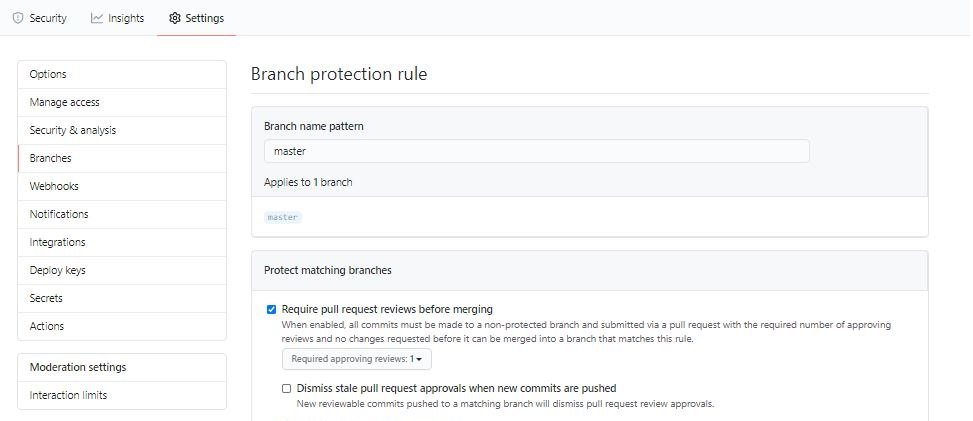
\includegraphics[scale = 1.0]{protected.jpg}
\end{center}


\item Далее создаете себе ветку (или ветки) для работы над проектом и его фичами, например, dev. И как только вы что-то хотите залить в master, то будет сформирован pull request, в котором надо будет указать меня в качестве reviewer-а.

При таком подходе, я смогу проследить за всеми изменениями и ничто не пройдет мимо моего взгляда. Для вас ветка dev будет аналогом master, в которую вы можете лить все, что угодно. А вот master будет копией dev, в которую лить можно только после моего одобрения и проверки. У себя на машине вы можете иметь миллион локальных веток для работы и организации фичей.

\item При инициализации проекта я бы рекомендовал первым делом не писать код, а настроить следующее:
\begin{enumerate}
\item Файл \verb".gitignore". У самого github есть куча разных шаблонов \verb".gitignore" для разных проектов и для плюсов и для \LaTeX и для много чего еще. Можно у них своровать. Я обычно делаю закрытый временный репозиторий, инициализирую его с \verb".gitignore" для нужного шаблона, а потом из него копирую себе github-овский \verb".gitignore". Может быть можно как-то проще их оттуда достать, но так работает.

\item Написание readme файла с указанием в нем названия проекта, а так же в дальнейшем можно в него помещать описание сборки проекта и инструкций к действию.

\item Для плюсовых проектов настроить \href{https://clang.llvm.org/docs/ClangFormatStyleOptions.html}{файл} \verb".clang-format".
\end{enumerate}

\item Если вам нужны какие-то сторонние библиотеки, то часто они уже есть на github и их можно использовать с помощью git submodules. Хороший текст для понимания вот \href{https://git-scm.com/book/en/v2/Git-Tools-Submodules}{тут}, а референс по командам \href{https://git-scm.com/docs/git-submodule}{тут}.
\end{enumerate}

\appendix

\section{Примеры вставок кода}

Этот кусочек посвящен примерам вставки кода в \LaTeX. Я для этого собрал свое собственное окружение на основе listings package.

\paragraph{Вставка из файла}

Можно добавить код из файла, указав с какой строчки по какую вы добавляете.
\inputcppcode[firstline=106, lastline=115]{AnyMovable.h}
Если надо выдрать не непрерывно идущий кусок из строк, то можно указать семейство диапазонов.
\inputcppcode[linerange={98-100,247-247}]{AnyMovable.h}

\paragraph{Набор кода вручную}

Здесь пример того, как можно написать свой собственный кусок кода прям в \LaTeX. В нем демонстрируется вся поддерживаемая подсветка синтаксиса.
\begin{cppcode}
#include <math.h>

char * str = "for if then some string! i = 0 ";

/*
Comment
*/

class Complex {
public:
  Complex(double re, double im)
    : _re(re), _im(im) {
  }
  double modulus() const {
    return sqrt(_re * _re + _im * _im);
  }
private:
  double _re;
  double _im;
};

void bar(int i) {
  static int counter = 0;
  counter += i;
}

namespace Foo {
namespace Bar {
void foo(int a, int b) {
  for (int i = 0; i < a; i++) {
    if (i < b)
      bar(i);
    else {
      bar(i);
      bar(b);
    }
  }
}
} // namespace Bar
} // namespace Foo
\end{cppcode}

\paragraph{Стиле ключевых слов}

Для удобства ниже приведены стили для ключевых слов. По сути сейчас из множества ключевых слов выделены типы переменных, которые отображаются голубым, остальные -- оранжевым. Все это можно перенастроить в файле code.sty. Даже можно добавить свои новые классы ключевых слов, как вам вздумается и выбрать для них свой способ отображения.
\begin{cppcode}
alignas,
alignof,
and,
and_eq,
asm,
atomic_cancel,
atomic_commit,
atomic_noexcept,
auto,
bitand,
bitor,
bool,
break,
case,
catch,
char,
char8_t,
char16_t,
char32_t,
class,
compl,
concept,
const,
consteval,
constexpr,
constinit,
const_cast,
continue,
co_await,
co_return,
co_yield,
decltype,
default,
delete,
do,
double,
dynamic_cast,
else,
enum,
explicit,
export,
extern,
false,
float,
for,
friend,
goto,
if,
inline,
int,
long,
mutable,
namespace,
new,
noexcept,
not,
not_eq,
nullptr,
operator,
or,
or_eq,
private,
protected,
public,
reflexpr,
register,
reinterpret_cast,
requires,
return,
short,
signed,
sizeof,
static,
static_assert,
static_cast,
struct,
switch,
synchronized,
template,
this,
thread_local,
throw,
true,
try,
typedef,
typeid,
typename,
union,
unsigned,
using,
virtual,
void,
volatile,
wchar_t,
while,
xor,
xor_eq,
\end{cppcode}


% Здесь текст документа заканчивается
\end{document}
% Начиная с этого момента весь текст LaTeX игнорирует, можете вставлять любую абракадабру.
